\documentclass[10pt]{article}
\usepackage[italian]{babel}
\usepackage{array}
\usepackage{graphicx}
\usepackage[export]{adjustbox}
\usepackage{ragged2e}
\usepackage{float}
\usepackage[hidelinks]{hyperref}
\usepackage{caption}

\setlocalecaption{italian}{contents}{Indice}

\begin{document}

\par\medskip
\begin{center}

\includegraphics[scale=0.1,center]{unifilogo/firenze2}
\end{center}

\begin{center}
\par\medskip
\textsc{{\large Università degli studi di Firenze}}\\
\par\medskip
\textsc{{\normalsize Dipartimento di Ingegneria Informatica}}\\
\par\medskip
\par\medskip
\hrule width 12cm height 1pt \par
\par\medskip
\par\medskip
\par\medskip
{\Huge \textbf{Apartament}}\\
\par\medskip
\par\medskip
\par\medskip
\hrule width 12cm height 1pt \par
\par\medskip
\par\medskip
{\Large \textbf{Link Github: \href{https://github.com/Pennelli02/SweProject}{https://github.com/Pennelli02/SweProject}}}
\par\medskip
\par\medskip
\hrule width 12cm height 1pt \par
\par\medskip
\par\medskip
\par\medskip
\emph{Autori:} \hfill \emph{Docente corso:}\\
\par\medskip
Pennelli Lorenzo Maria \hfill Vicario Enrico\\
\begin{FlushLeft}
Leuter Lorenzo\\
\end{FlushLeft}

\end{center}

\newpage

\tableofcontents

\newpage

\section{Introduzione}

\subsection{Descrizione del progetto}

L'obiettivo è creare un'applicazione java che permetta di gestire le prenotazioni di alloggi, in particolare verranno trattati B\&B, appartamenti e hotel. Gli utenti avranno la possibilità di effettuare ricerche e prenotazioni degli alloggi disponibili, selezionare il numero di persone che soggiorneranno, la data di inizio e di fine del soggiorno, e molti altri filtri che verranno spiegate successivamente. Inoltre, l'utente potrà anche cancellare le prenotazione se necessario, poter inserire tra i preferiti gli alloggi e lasciare delle recensioni degli alloggi da loro prenotati in precedenza.\`E inoltre presente un Admin che può cancellare definitivamente gli utenti o recensioni, aggiungere nuovi alloggi, modificare gli alloggi già presenti oppure rimuoverli.

\subsection{Ambiente di sviluppo, Architettura del progetto e pratiche usate}

L'applicazione è stata sviluppata nel linguaggio Java e il database è stato implementato con PostrgreSQL. La connessione tra il progetto e il database è realizzata tramite JDBC. L'architettura del progetto è rappresentata dalla figura sottostante: 
\begin{center}
\hspace*{-1cm}
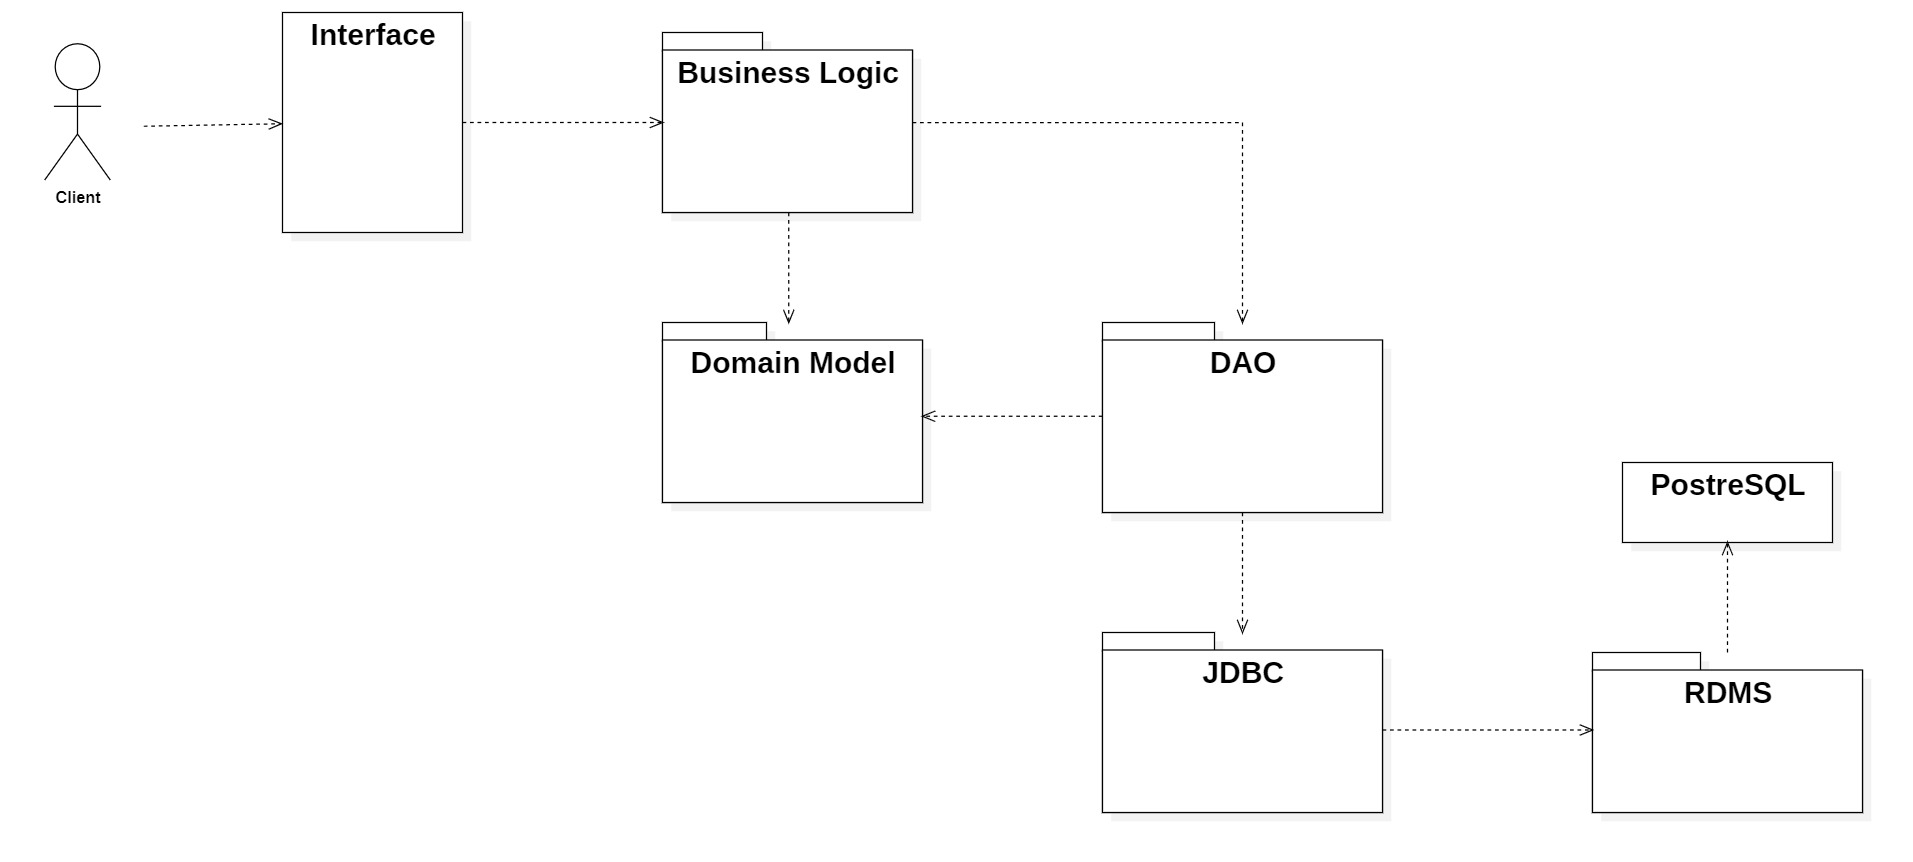
\includegraphics[scale=0.175]{Sp/Architettura}
\par\medskip
Figura 1: Diagramma dell'architettura del progetto
\par\medskip
\end{center}
L'architettura del progetto è articolata in tre componenti:
\begin{itemize}
	\item \textbf{Business Logic}: contiene le classi che implementano la logica di business nel sistema.
	\item \textbf{Domain Model}: contiene le classi che rappresentano le entità del sistema.
	\item \textbf{DAO}: contiene le classi che permettono di gestire la comunicazione tra l'applicazione e il database andando a separare la logica per l'interazione con i dati dal resto dell'applicazione.
\end{itemize}
Infine per l'uso del software e l'interazione con il sistema è stata creata un'interfaccia a linea di comando (CLI).\\
Sono state utilizzate le seguenti piattaforme e software:
\begin{itemize}
\item \textbf{IntelliJ IDEA}: IDE per lo sviluppo in Java.
\item \textbf{StarUML}: software per la creazione di diagrammi UML.
\item \textbf{Draw.io}: software per la realizzazione di altri diagrammi, tra cui il modello ER.
\item \textbf{PgAdmin}: software per la gestione del database PostgreSQL.
\item \textbf{GitHub}: piattaforma contenente il codice sorgente.
\item \textbf{Lunacy}: software per la realizzazione dei mockup.
\end{itemize}


\section{Progettazione}
\subsection{Use Case Diagram}

Sono presenti 2 tipi di utenti: lo User e l'Admin. Nel diagramma sottostante vengono rappresentati i casi d'uso per i due tipi di utenti: 

\begin{center}
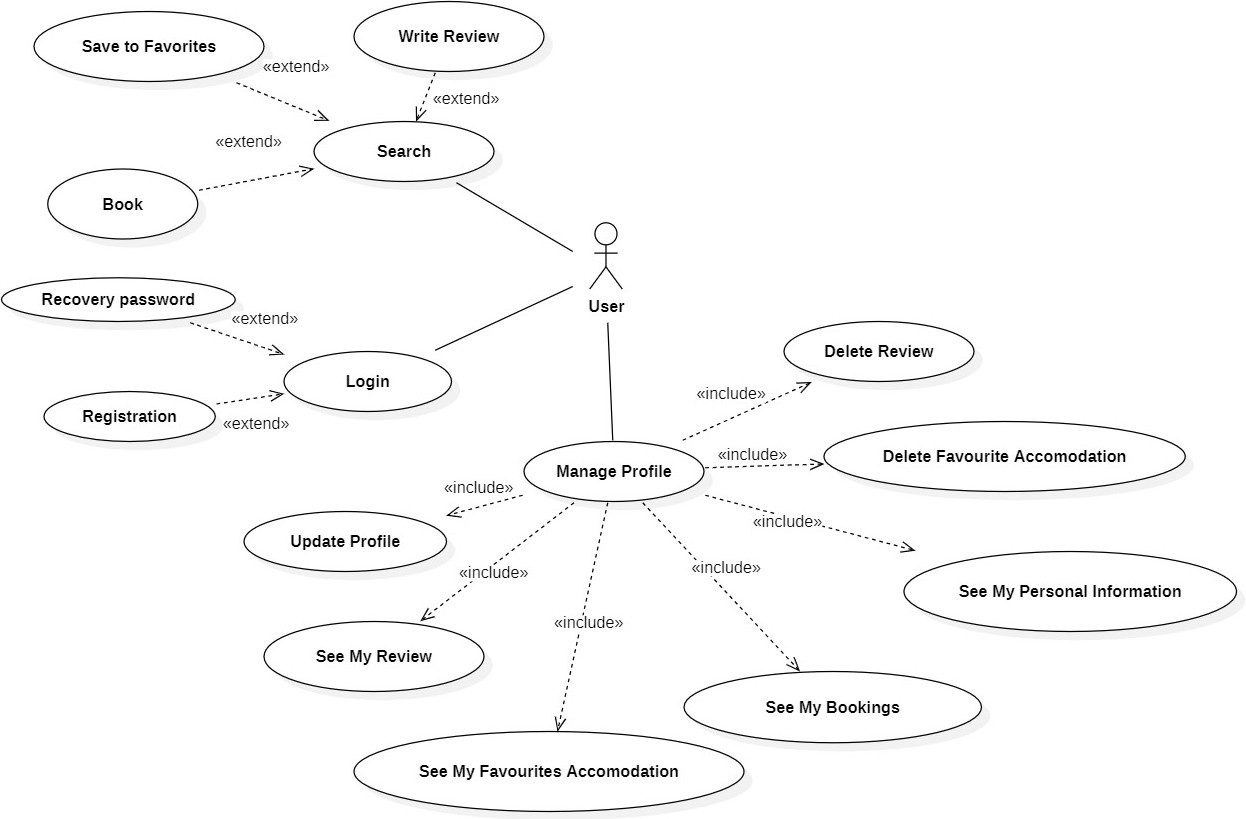
\includegraphics[scale=0.411]{usecases/ClientUseCase}
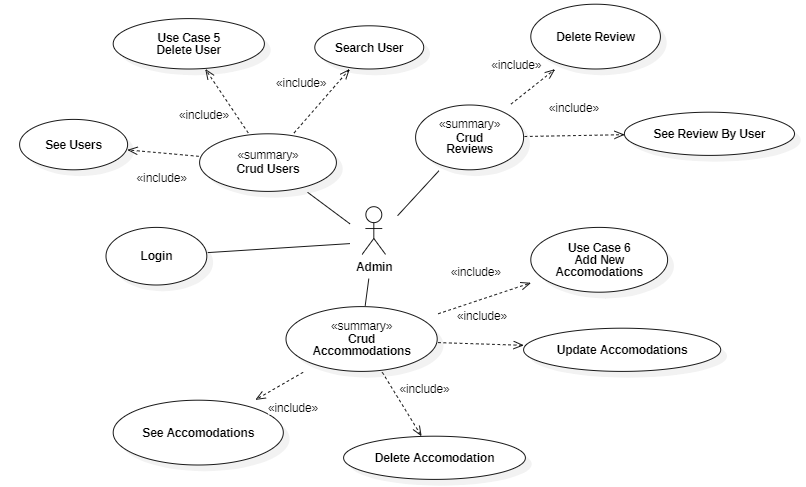
\includegraphics[scale=0.5]{usecases/AdminUseCase}\\
Figura 2: Use Case Diagram dello User e dell'Admin
\end{center}

\subsection{Use Case Template}
Sono di seguito alcuni template dei casi d'uso. In alcuni di essi sono presenti riferimenti a mockup presenti successivamente (sezione 2.3):

\begin{center}
\begin{table}[H]
\vspace{-0.3cm}
\centering
\scalebox{0.75}{ % Riduce tutto il blocco al 75% della dimensione originale
\begin{tabular}{|l|p{9cm}|}
\hline
Use Case 1 & Login \\ \hline
Descrizione & L'utente accede al sistema inserendo le sue credenziali. \\ \hline
Livello & Function \\ \hline
Attori & Utente, Admin \\ \hline
Flusso Base & 
\begin{enumerate}
    \item L'utente inserisce le sue credenziali (email e password) (\hyperref[mk1]{MK\#1} e \hyperref[mk3]{MK\#3}).
    \item L'utente preme il pulsante di Login.
    \item Il sistema verifica le credenziali.
    \item Il sistema autentica l'utente.
\end{enumerate} \\ \hline
Flusso Alternativo & 
\begin{enumerate}
    \item[3a.] Se le credenziali sono errate, il sistema invia un messaggio di errore.
    \item[3b.] Se si verifica un problema all'interno del database durante la ricerca dell'utente, il sistema invia un messaggio di errore.
    \item[4a.] Se l'accesso viene effettuato dall'utente, sarà indirizzato alla sua pagina personale.
\end{enumerate} \\ \hline
Post-condizioni & L'utente è autenticato dal sistema e ha accesso alle sue funzionalità. \\ \hline
\end{tabular}
}
\caption{Template che descrive il caso d'uso del login}
\end{table}
\begin{table}[H]
\vspace{-0.3cm}
\centering
\scalebox{0.75}{ % Riduce tutto il blocco al 75% della dimensione originale
\begin{tabular}{|l|p{9cm}|}
\hline
Use Case 2 & Search \\ \hline
Descrizione & L'utente cerca l'alloggio di suo interesse. \\ \hline
Livello & User Goal \\ \hline
Attori & User \\ \hline
Flusso Base & 
\begin{enumerate}
    \item L'utente inserisce le informazioni per effettuare la sua ricerca (\hyperref[mk6]{MK\#6}).
    \item L'utente preme il pulsante per effettuare la ricerca.
    \item Il sistema usa le informazioni per ricercare gli alloggi.
    \item Il sistema restituisce all'utente una lista di alloggi (\hyperref[mk7]{MK\#7}).
\end{enumerate} \\ \hline
Flusso Alternativo & 
\begin{enumerate}
    \item[3a.] Se l'utente non inserisce alcune informazioni necessarie alla ricerca (es: il luogo dove vuole andare, la data di check-in, la data di check-out), il sistema restituisce un messaggio di errore.
    \item[3b.] Se si verifica un problema all'interno del database durante la ricerca dell'alloggio, il sistema invia un messaggio di errore.
\end{enumerate} \\ \hline
Pre-condizioni & L'utente deve aver fatto il login. \\ \hline
Post-condizioni & L'utente riceverà una lista di alloggi da consultare. \\ \hline
\end{tabular}
}
\caption{Template che descrive il caso d'uso dello Research}
\end{table}
\begin{table}[H]
\vspace{-0.3cm}
\centering
\scalebox{0.75}{ % Riduce tutto il blocco al 75% della dimensione originale
\begin{tabular}{|l|p{9cm}|}
\hline
Use Case 3 & Book \\ \hline
Descrizione & L'utente prenota un alloggio. \\ \hline
Livello & User Goal \\ \hline
Attori & User \\ \hline
Flusso Base & 
\begin{enumerate}
    \item L'utente preme il pulsante per effettuare la prenotazione dell'alloggio (\hyperref[mk2]{MK\#2}).
    \item Il sistema riceve la richiesta di prenotazione e verifica la disponibilità dell'alloggio.
    \item Il sistema restituisce all'utente un messaggio di conferma.
\end{enumerate} \\ \hline
Flusso Alternativo & 
\begin{enumerate}
    \item[2a.] Se la disponibilità è zero, il sistema restituisce un messaggio di errore.
    \item[2b.] Se si verifica un problema durante il salvataggio della prenotazione nel database, il sistema invia un messaggio di errore.
\end{enumerate} \\ \hline
Pre-condizioni & L'utente deve aver fatto il login e deve aver effettuato la ricerca. \\ \hline
Post-condizioni & La prenotazione effettuata verrà aggiunta a quelle già effettuate dell'utente. \\ \hline
\end{tabular}
}
\caption{Template che descrive il caso d'uso del Book}
\end{table}
\begin{table}[H]
\vspace{-0.3cm}
\centering
\scalebox{0.75}{ % Riduce tutto il blocco al 75% della dimensione originale
\begin{tabular}{|l|p{9cm}|}
\hline
Use Case 4 & Registration \\ \hline
Descrizione & L’utente si registra all’interno del sistema. \\ \hline
Livello & User Goal \\ \hline
Attori & User \\ \hline
Flusso Base & 
\begin{enumerate}
    \item L'utente inserisce i parametri per registrarsi (\hyperref[mk5]{MK\#5}).
    \item L'utente preme il pulsante per effettuare la registrazione.
    \item Il sistema verifica le informazioni fornite.
    \item Il sistema crea un nuovo account per l’utente.
\end{enumerate} \\ \hline
Flusso Alternativo & 
\begin{enumerate}
    \item[3a.] Se l’utente inserisce dati non validi (es: l’email/username già usati), il sistema invia un messaggio di errore all’utente.
    \item[3b.] Se si verifica un problema durante il salvataggio dell’utente nel database, il sistema invierà un messaggio di errore.
\end{enumerate} \\ \hline
Post-condizioni & L’utente è registrato all’interno del sistema e può accedere tramite le sue credenziali. \\ \hline
\end{tabular}
}
\caption{Template che descrive il caso d'uso del Registration}
\end{table}
\begin{table}[H]
\vspace{-0.3cm}
\centering
\scalebox{0.75}{ % Riduce tutto il blocco al 75% della dimensione originale
\begin{tabular}{|l|p{9cm}|}
\hline
Use Case 5 & Delete User \\ \hline
Descrizione & L'Admin elimina un utente dal database. \\ \hline
Livello & User Goal \\ \hline
Attori & Admin \\ \hline
Flusso Base & 
\begin{enumerate}
    \item L'admin inserisce i parametri che caratterizzano l'utente (es: username o email).
    \item L'admin preme il pulsante per effettuare l'eliminazione dell'utente.
    \item Il sistema verifica le informazioni fornite.
    \item Il sistema elimina l'utente dal database.
\end{enumerate} \\ \hline
Flusso Alternativo & 
\begin{enumerate}
    \item[3a.] Se l'admin inserisce dati non validi, il sistema invia un messaggio di errore.
    \item[3b.] Se si verifica un problema durante l'eliminazione dell'utente dal database, il sistema invierà un messaggio di errore.
\end{enumerate} \\ \hline
Pre-condizioni & L'admin deve aver effettuato il login. \\ \hline
Post-condizioni & L'utente è stato eliminato con successo e non può più accedere all'applicazione a meno che non venga effettuata una nuova registrazione. \\ \hline
\end{tabular}
}
\caption{Template che descrive il caso d'uso del Delete User}
\end{table}
\begin{table}[H]
\centering
\scalebox{0.75}{ % Riduce tutto il blocco al 75% della dimensione originale
\begin{tabular}{|l|p{9cm}|}
\hline
Use Case 6 & Add Accommodation \\ \hline
Descrizione & L'admin aggiunge un nuovo alloggio al database. \\ \hline
Livello & User Goal \\ \hline
Attori & Admin \\ \hline
Flusso Base & 
\begin{enumerate}
    \item L'admin inserisce i parametri che caratterizzano l'alloggio.
    \item L'admin preme il pulsante per effettuare l'aggiunta dell'alloggio.
    \item Il sistema verifica le informazioni fornite.
    \item Il sistema registra l'alloggio appena inserito.
\end{enumerate} \\ \hline
Flusso Alternativo & 
\begin{enumerate}
    \item[3b.] Se si verifica un problema durante la registrazione dell'alloggio nel database, il sistema invia un messaggio di errore.
\end{enumerate} \\ \hline
Pre-condizioni & L'admin deve aver fatto il login. \\ \hline
Post-condizioni & L'alloggio è stato registrato con successo e sarà disponibile per le successive ricerche degli utenti. \\ \hline
\end{tabular}
}
\caption{Template che descrive il caso d'uso dell'Add Accomodation}
\end{table}
\end{center}


\subsection{Mockups}
Sono riportati alcuni mockup, realizzati con \textbf{Lunacy}, relativi ad una possibile interfaccia grafica per l'applicazione:
\begin{center}
\phantomsection
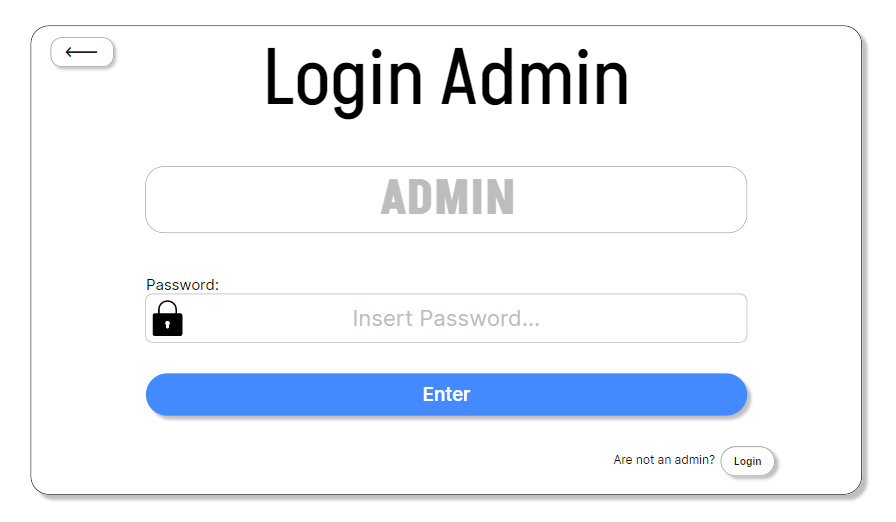
\includegraphics[scale=0.6]{Mockup/MockupAdminLogin}
\label{mk1}
\par\medskip
Figura 3: Mockup per il login effettuato da un admin - MK\#1 
\par\medskip
\par\medskip
\phantomsection
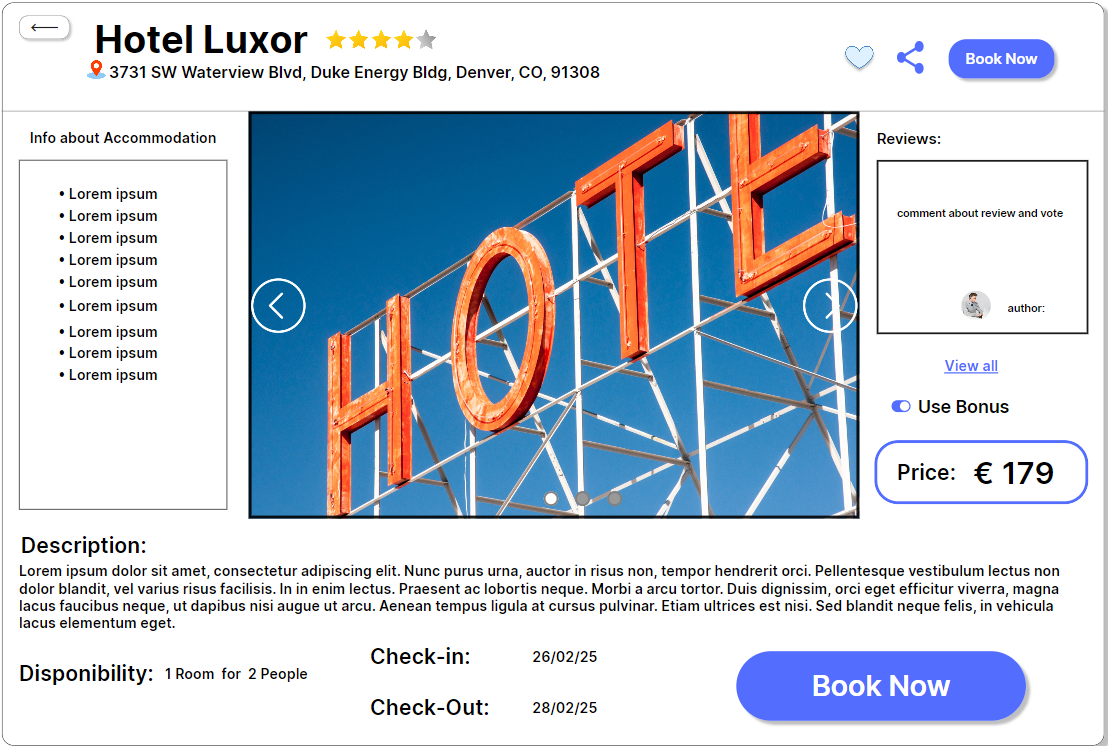
\includegraphics[scale=0.5]{Mockup/mockupBooking}
\label{mk2}
\par\medskip
\par\medskip
Figura 4: Mockup per mostrare in dettaglio un alloggio con la possibilità di prenotarlo - MK\#2
\par\medskip
\phantomsection
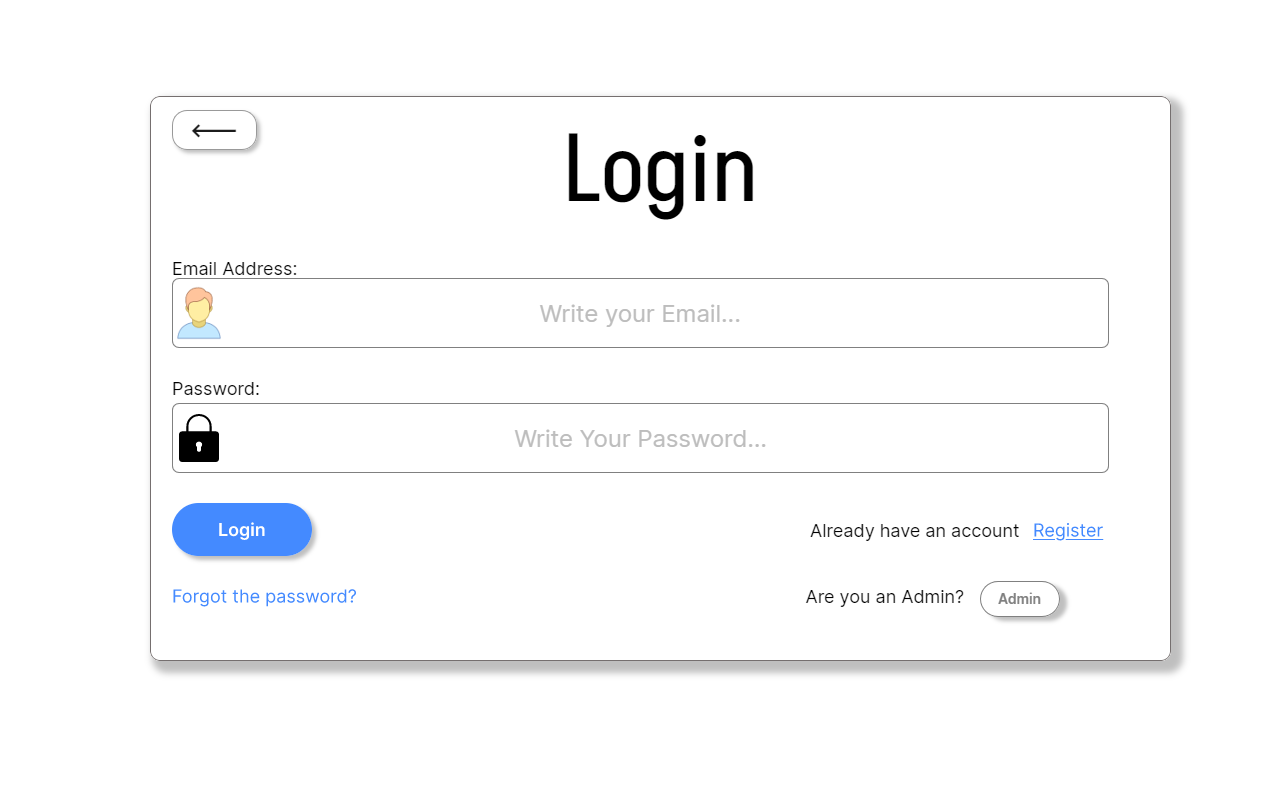
\includegraphics[scale=0.5]{Mockup/MockupLogin}
\label{mk3}
\par\medskip
Figura 5: Mockup per il login effettuato da un utente - MK\#3
\par\medskip
\phantomsection
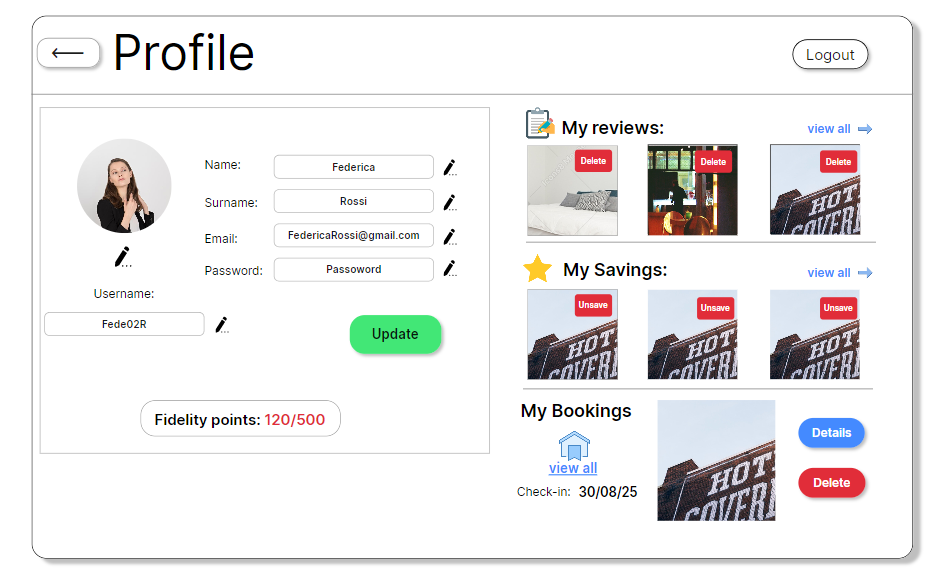
\includegraphics[scale=0.6]{Mockup/MockupProfile}
\label{mk4}
\par\medskip
Figura 6: Mockup per mostrare il profilo di un utente - MK\#4
\par\medskip
\phantomsection
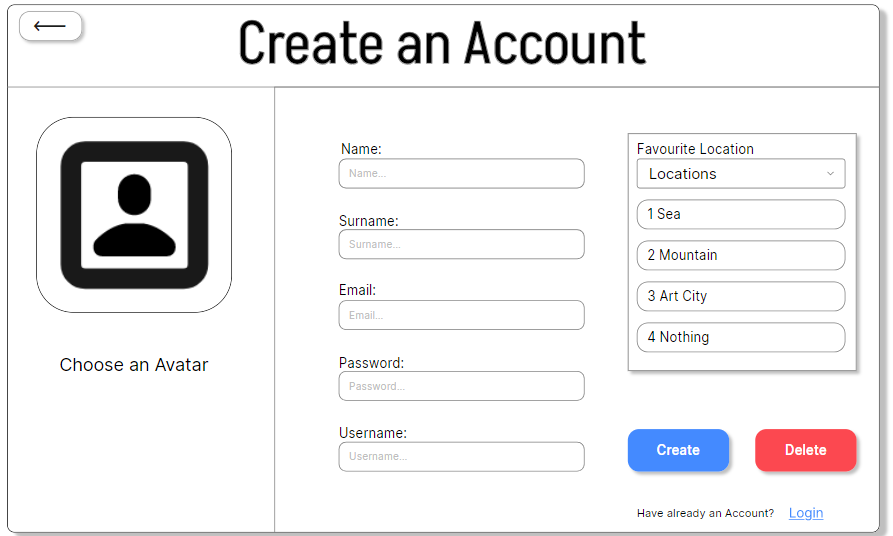
\includegraphics[scale=0.6]{Mockup/MockupRegister}
\label{mk5}
\par\medskip
\par\medskip
Figura 7: Mockup per creare un account - MK\#5
\par\medskip
\par\medskip
\phantomsection
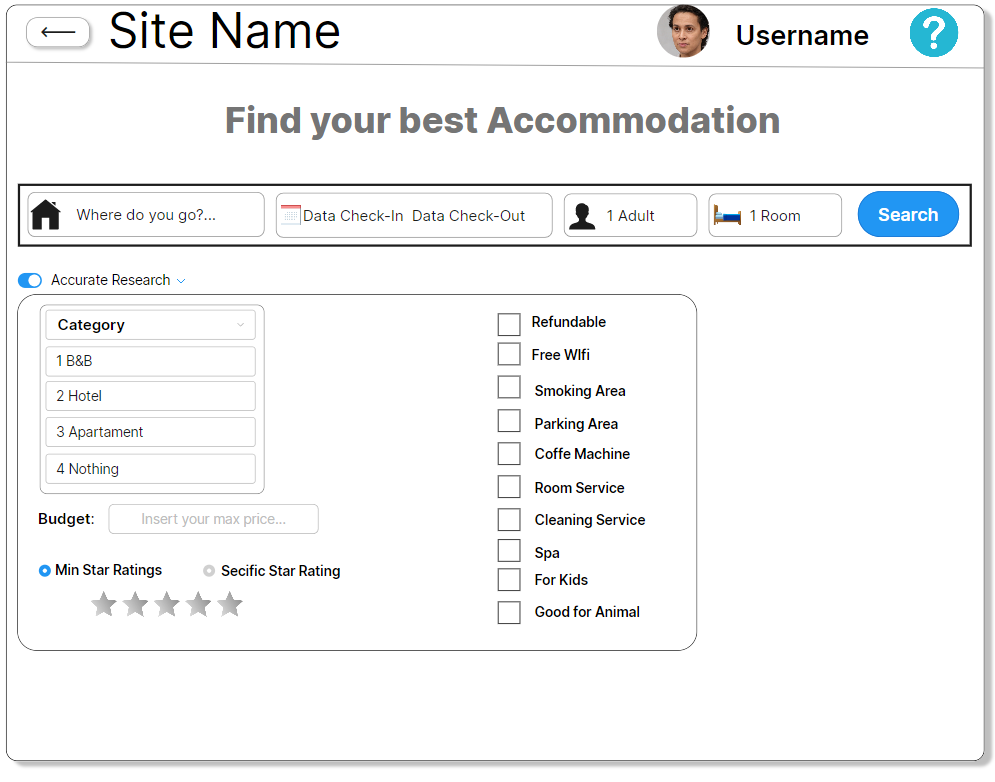
\includegraphics[scale=0.55]{Mockup/MockupResearch}
\label{mk6}
\par\medskip
Figura 8: Mockup per effettuare la ricerca attraverso i filtri - MK\#6
\par\medskip
\phantomsection
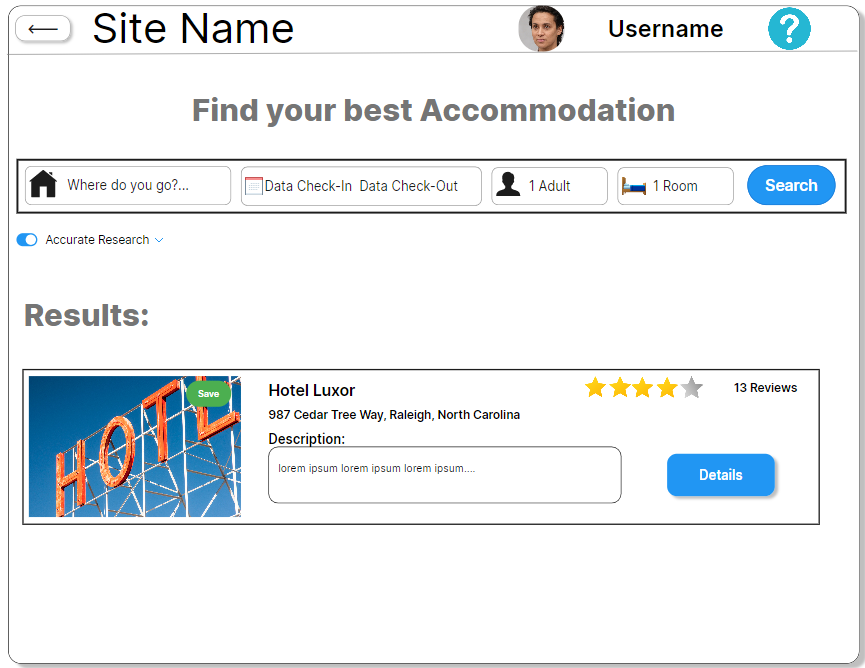
\includegraphics[scale=0.6]{Mockup/MockupResult}
\label{mk7}
\par\medskip
Figura 9: Mockup che mostra i risualtati di una ricerca - MK\#7
\par\medskip
\end{center}

\subsection{Class Diagram}
L'architettura è divisa in 3 package:
\begin{itemize}
\item \textbf{Business Logic}:è il package che contiene i controller, che sono 4: quello che gestisce l'accesso, la registrazione e l'eliminazione degli utenti (\textbf{UserController}), quello che gestisce il profilo dell'utente (\textbf{ProfileUserController}), quello che gestisce la logica dell'applicazione (ricerca,prenotazione,recensione) (\textbf{ResearchController}) e quello che gestisce le azioni che può effettuare l'Admin (\textbf{AdminController}). 
\vspace{-0.3cm}
\par\medskip
\hspace*{-0.75cm}
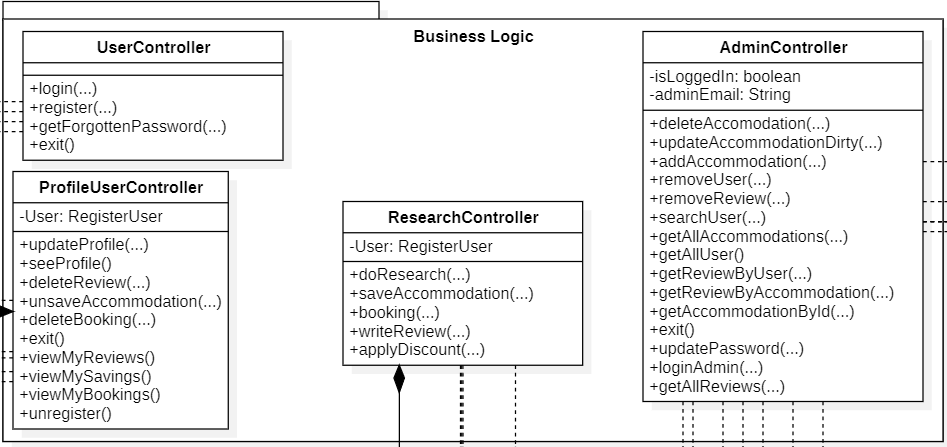
\includegraphics[scale=0.6]{uml/BusinessLogic}
\begin{center}
Figura 10: Class Diagram - Business Logic 
\end{center}
\item \textbf{Domain Model}: consiste nell’insieme di classi che rappresentano i concetti con cui interagisce l’applicazione: \textbf{RegisterUser}, \textbf{Review}, \textbf{Booking}, \textbf{Accommodation}, \textbf{SearchParameters},\textbf{SearchParametersBuilder}.
\hspace*{-2cm}
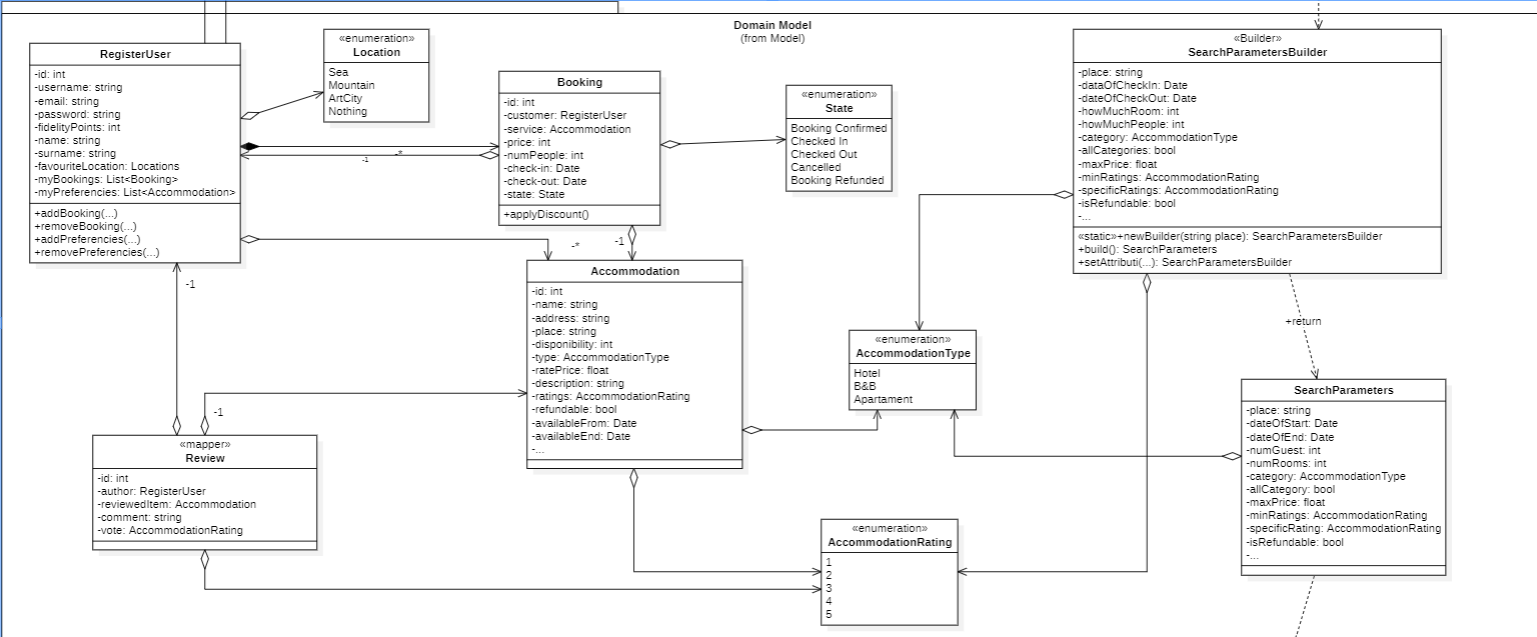
\includegraphics[scale=0.58]{uml/domainModel}
\par\medskip
\begin{center}
Figura 11: Class Diagram - Domain Model 
\end{center}
\par\medskip
\vspace{-0.3cm}
\item \textbf{DAO}: è il package che si occupa di gestire la connessione con il database: \textbf{UserDAO}, \textbf{BookingDAO}, \textbf{PreferenceDAO}, \textbf{ReviewDAO}, \textbf{AccommodationDAO}, \textbf{DatabaseConnection}.
\vspace{0.1cm}
\par\medskip
\hspace*{-0.5cm}
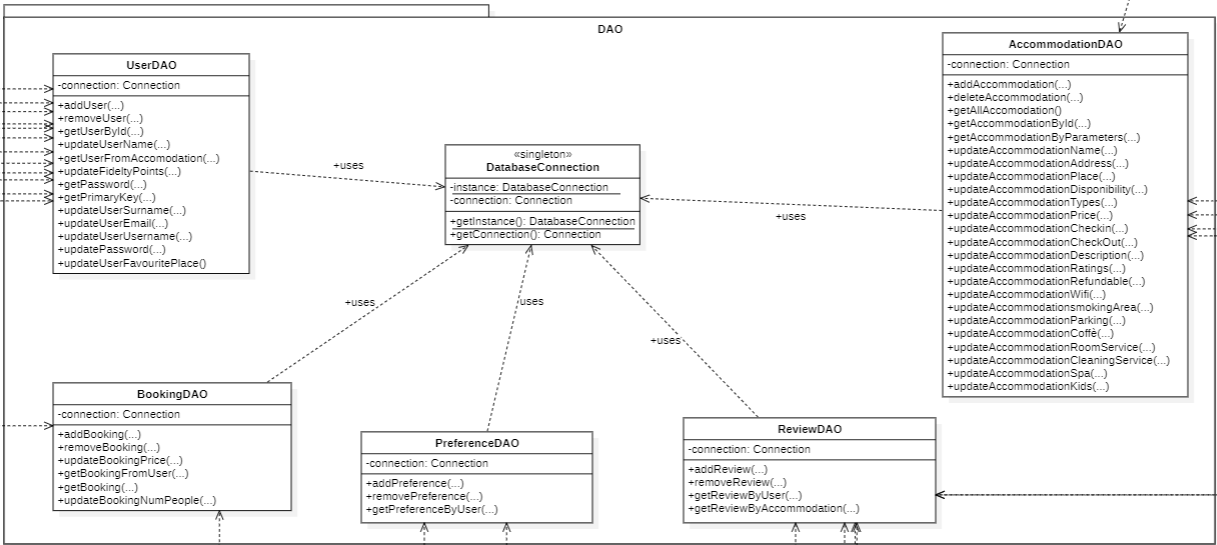
\includegraphics[scale=0.58]{uml/DAO}
\par\medskip
\begin{center}
Figura 12: Class Diagram - DAO
\end{center}
\par\medskip
\end{itemize}
\subsection{Dettagli di Progetto}
Nell'architettura sono stati usati diversi design pattern:
\subsubsection{Singleton}

Lo scopo del Singleton è stato utilizzato per garantire che la connessione al database venisse effettuata una singola volta e per evitare conflitti tra connessioni.
\vspace{-0.3cm}
\begin{center}
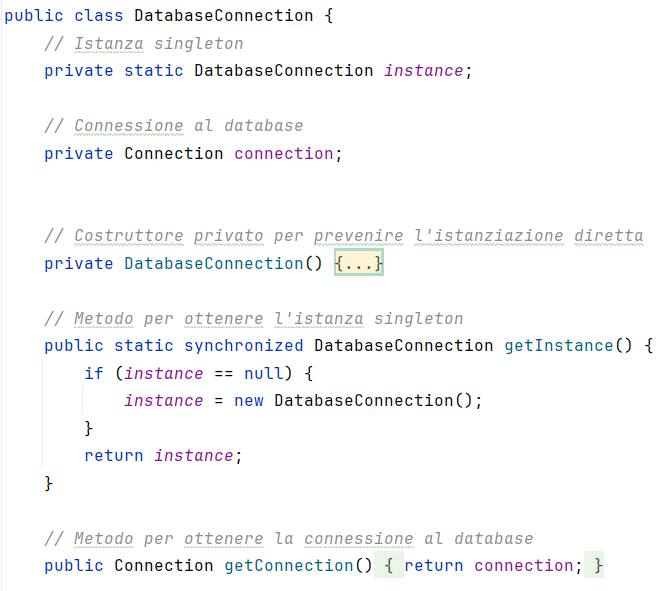
\includegraphics[scale=0.45]{Snippets/Singleton}
\par\medskip
Snippet 1: Implementazione Singleton
\par\medskip
\end{center}

\subsubsection{Mapper}

Lo scopo del Mapper è quello di creare la relazione tra utenti, recensioni e alloggi.

\begin{center}
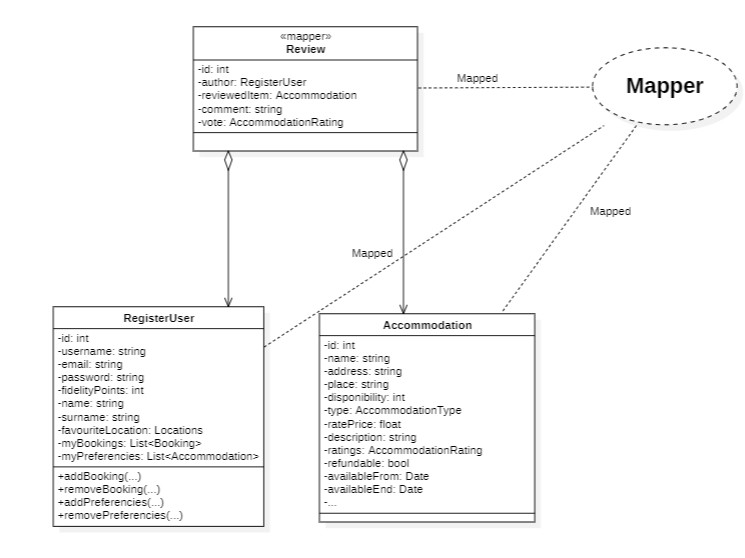
\includegraphics[scale=0.85]{Snippets/Mapper}
\par\medskip
Snippet 2: UML del Mapper
\par\medskip
\end{center}

\subsubsection{Builder Telescoping Constructor}

Il Builder Telescoping Constructor viene usato per creare la classe parametri di ricerca che presenta tanti attributi, spesso opzionali, e consente una gestione più efficiente. L'unico scopo della classe è quello creare un oggetto di tipo ParametriRicerca e ci riesce grazie ai metodi di setting, che ritornando la classe stessa, consentono di avere una chiara creazione dell'oggetto, attraverso un metodo statico e evitando l'overloading dei costruttori tradizionale (\textbf{build}).

\subsubsection{DAO}

Il DAO (Data Access Object) è un design pattern che si occupa di separare le classi che si interfacciano al database dall'applicazione. Questo viene fatto
per poter meglio implementare il principio di singola responsabilità e aumenta
la mantenibilità del codice.

\subsection{ER Diagram e Relational Model}

Per il database e la sua gestione, è stato realizzato un ER Diagram (Figura 13), e il Relational Model derivato (Figura 14), entrambi realizzati con \textbf{Draw.io}. Ci sono state delle scelte progettuali precise, in particolare quella riguardante l'entità \textbf{Alloggio}, dove per differenziare i tipi di alloggio è stato usato un'attributo al posto di una generalizzazione, dovuto al fatto che nel progetto si faranno uso di informazioni che sono a comune tra i vari alloggi, favorendo accessi più veloci ma a discapito di un notevole spreco di memoria e la presenza di valori nulli.\\
Alla fine sono state definite le seguenti tabelle (Figura 15):
\begin{itemize}
\item \textbf{User}: rappresenta l'entità \textbf{User}.
\item \textbf{Booking}: rappresenta l'entità \textbf{Booking}.
\item \textbf{Acccommodation}: rappresenta l'entità \textbf{Accommodation}.
\item \textbf{Review}: rappresenta la relazione \textbf{Review} che avviene tra l'entità \textbf{User} e l'entità \textbf{Accommodation}.
\item \textbf{Favourites}: rappresenta la relazione \textbf{Like} che avviene tra l'entità \textbf{User} e l'entità \textbf{Accommodation}.
\end{itemize}
\begin{center}
\par\medskip
\hspace*{-2cm}
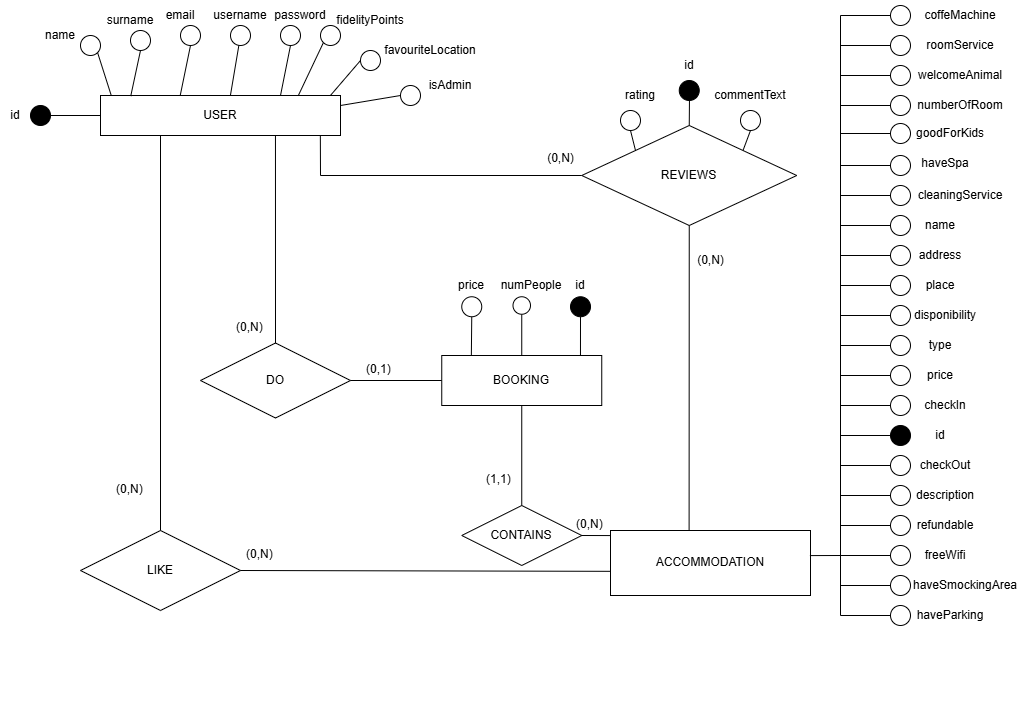
\includegraphics[scale=0.41]{ERImages/FinalER}
\par\medskip
Figura 13: ER Diagram
\par\medskip
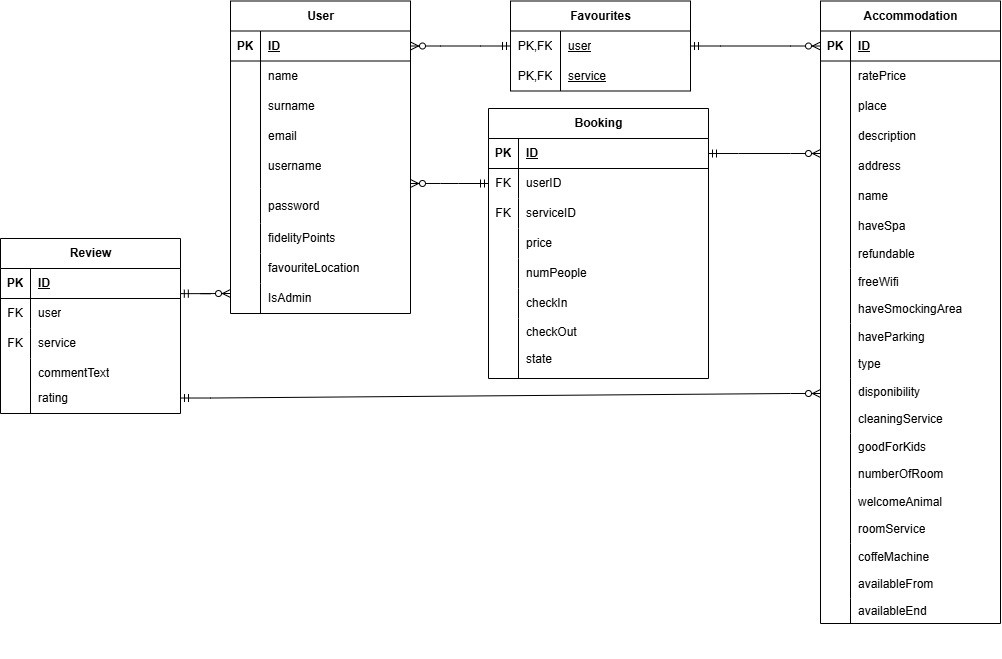
\includegraphics[scale=0.5]{ERImages/schemaLogicoDBTabelle}
\par\medskip
Figura 14: Tables of the database
\par\medskip
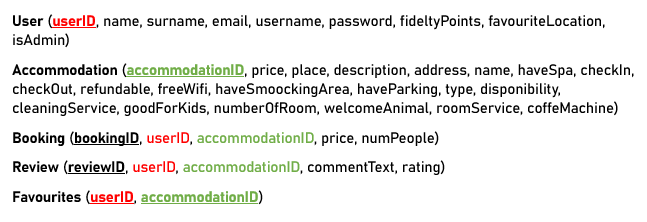
\includegraphics[scale=0.75]{ERImages/RelationalModel}
\par\medskip
Figura 15: Relation Model
\par\medskip
\end{center}

\section{Implementazione}
\subsection{Business Logic}

\`E il package che contiene i controller e che espone all'esterno le funzionalità dell'applicazione. \`E responsabilità dei controller gestire le dipendenze tra gli oggetti creati dai DAO.

\subsubsection{UserController}

\`E la classe che si occupa di implementare le funzionalità di un utente generico per l'accesso all'applicazione. Infatti presenta i metodi di login, di registrazione, cancellare l'utente in uso e un eventuale recupera password.

\subsubsection{ProfileController}

\`E la classe che si occupa di gestire le informazioni del profilo utente e dei servizi di cui ha usufruito (\textbf{deleteReview()}, \textbf{deleteBooking()}, \textbf{unsaveAccommodation()}, \textbf{viewMySavings()}, \textbf{viewMyReviews()}, \textbf{viewMyBookings()}).

\subsubsection{ResearchController}

\`E la classe che si occupa di fornire i metodi che implementano la logica dell'applicazione. Infatti, permette la ricerca in base a dei parametri (\textbf{doResearch()}) e sugli alloggi ricercati permette,a un utente registrato, di effettuare una prenotazione (\textbf{booking()}), salvarlo tra i preferiti (\textbf{saveAccomodation()}) e scrivere una recensione su quell'alloggio (\textbf{writeReview()}). Per funzionare, oltre ai collegamenti ai relativi DAO, questa classe usa il \textbf{SearchParametersBuilder} che si trova nel \textbf{Domain Model}.

\subsubsection{AdminController}

\`E la classe che si occupa di implementare le operazioni dell'admin, il quale può  leggere, modificare, cancellare e aggiungere alloggi, mentre può solo leggere e cancellare utenti e recensioni.
 
\subsection{Domain Model}

\`E il package che rappresenta il modello dei dati e implementa le classi che raffigurano le entità del sistema.

\subsubsection{RegisterUser}

Contiene le informazioni relative all'utente registrato. Gli attributi della classe sono: id (utilizzato come identificativo), username, email (unica all'interno dell'applicazione), password, nome, cognome, punti fedeltà (che si aggiornano ad ogni acquisto e raggiunta una certa soglia, permette di avere degli sconti), località preferita che indica un genere di esperienza che preferisce, la lista delle prenotazioni effettuate e la lista dei suoi alloggi preferiti. 

\subsubsection{Booking}

\`E la classe che rappresenta l'entità prenotazione, con tutte le informazioni relative ad essa. Possiede un id identificativo, l'acquirente, il servizio, per quante persone è la prenotazione, il prezzo, il check-in, il check-out e lo stato della prenotazione.

\subsubsection{Accommodation}

\`E la classe che rappresenta l'entità alloggio e tiene conto dei suoi attributi. Molti dei suoi attributi non sono obbligatori, ma possono essere nulli perché dipendono dai servizi che offre l'alloggio. Ha un id (univoco), un nome, un indirizzo, un luogo, quante persone possono alloggiarci, tipo di alloggio (B\&B, appartamento e hotel), il prezzo, il periodo di disponibilità, la descrizione di cosa offre, e diversi parametri aggiuntivi che non sono obbligatori (visualizzabili nelle figure precedenti).

\subsubsection{Review}

\`E la classe che rappresenta l'entità recensione. I campi sono id, autore, alloggio recensito, commento e il voto. Consente di stabilire una correlazione tra l'utente e l'alloggio in maniera discreta, senza che tale connessione sia direttamente percepita dagli interessati.

\subsubsection{SearchParametersBuilder e SearchParameters}

Queste classi implementano il design pattern Builder Telescopic Constructor per la creazione dei parametri di ricerca. Il \textbf{SearchParametersBuilder} consente una creazione più facile da gestire e da estendere dei parametri di ricerca. Infatti il suo unico scopo è di creare la classe \textbf{SearchParameters}. Quest'ultima classe possiede solo gli attributi che poi serviranno alla ricerca all'interno del database. Gli attributi sono per la maggior parte uguali alla classe \textbf{Accommodation}.

\subsection{DAO}

\`E il package che implementa l'omonimo design pattern descritto nella sezione 2.5.4. Le classi in questo package permettono alle classi presenti nella \textbf{Business Logic} di accedere ai vari dati di loro interesse.

\subsubsection{DatabaseConnection}

\`E la classe che si occupa di gestire la connessione al database per le altre classi DAO tramite il metodo \textbf{getConnection()}. Classe implementata usando il design pattern \textit{Singleton} per evitare conflitti tra connessioni.

\subsubsection{UserDAO}

\`E la classe che si occupa della gestione dei dati degli utenti. Questa classe contiene molti metodi, offrendo la possibilità di aggiungere nuovi utenti e di rimuovere quelli già presenti nel database (rispettivamente \textbf{addUser()} e \textbf{removeUser()}), la possibilità di recuperare un utente tramite l'id identificativo (\textbf{getUserById()}) oppure tramite lo username (\textbf{getUserByUsername()}) o anche in altri modi.Infine la classe presenta i metodi che permettono di aggiornare i dati personali di un utente.

\subsubsection{BookingDAO}

\`E la classe che si occupa della gestione dei dati che riguardano le prenotazioni effettuate dagli utenti. La classe mette a disposizione metodi che permetto di aggiungere o rimuovere delle prenotazioni (rispettivamente \textbf{addBooking()} e \textbf{removeBooking()}), di visualizzare le prenotazioni fatte da uno specifico utente (\textbf{getBookingFromUser()}) o vederle tutte. Quest'ultimo metodo viene utilizzato da un admin per effettuare dei controlli e modifiche se fosse necessario.

\subsubsection{PreferenceDAO}

\`E la classe che si occupa della gestione dei dati che riguardano le liste di alloggi preferiti dagli utenti, i quali posso essere visionati senza dover fare una nuova ricerca. Questa classe contiene i metodi che permettono di aggiungere un nuovo alloggio tra i preferiti (\textbf{addPreference()}), di rimuovere un alloggio tra i preferiti (\textbf{removePreference()}) e di visualizzare gli alloggi preferiti di uno specifico utente (\textbf{getPreferenceByUser()}). 

\subsubsection{ReviewDAO}

\`E la classe che si occupa della gestione delle recensioni scritte sugli alloggi da parte degli utenti. La classe contiene i metodi che permettono di aggiungere nuove recensioni (\textbf{addReview()}), di rimuovere le recensioni dall'applicazione (\textbf{removeReview()}), e di visualizzare le recensioni scritte da uno specifico utente (\textbf{getReviewByUser()}) o visualizzare le tutte le recensioni scritte su uno specifico alloggio (\textbf{getReviewByAccommodation()}). 

\subsubsection{AccommodationDAO}

\`E la classe che si occupa della gestione dei dati degli alloggi. questa classe presenta molti metodi, permettendo di aggiungere nuovi alloggi (\textbf{addAccommodation()}), di rimuovere gli alloggi già presenti (\textbf{deleteAccommodation()}), di visualizzare tutti gli alloggi (\textbf{getAllAccommodation()}), di visualizzare uno nello specifico tramite il suo identificativo (\textbf{getAccommodationById()}, questo metodo è molto utile per la gestione degli alloggi da parte dell'admin) e di visualizzare gli alloggi che vengono ricercati tramite l'uso dei filtri (\textbf{getAccommodationByParameters()}). Infine sono presenti i metodi che permettono di aggiornare i dati di un alloggio. 


\end{document}
